\documentclass[a4paper,12pt]{article}
\usepackage{graphicx}

\usepackage{epstopdf}
\usepackage{gensymb}
\usepackage{float}
\usepackage{mathtools}
\usepackage{setspace}
\usepackage{tabularx}
\usepackage{svg}

\title{Designspecifikation}
%% Definitioner för LIPS-dokument

\usepackage[swedish]{babel}
\usepackage[utf8]{inputenc}
\usepackage[T1]{fontenc}
\usepackage{times}
\usepackage{ifthen}
\usepackage[labelfont=it]{caption}

\usepackage[margin=25mm]{geometry}

\def\arraystretch{1.6}

\usepackage{fancyhdr}
\pagestyle{fancy}
\lhead{}
\chead{\LIPSprojekttitel}
\rhead{\LIPSdatum}
\lfoot{\LIPSkursnamn \\ \LIPSdokumentansvarig}
\rfoot{\LIPSprojektgrupp \\ \LIPSgruppepost}

\setlength{\parindent}{0pt}
\setlength{\parskip}{1ex plus 0.5ex minus 0.2ex}


\newcommand{\twodigit}[1]{\ifthenelse{#1<10}{0}{}{#1}}
\newcommand{\dagensdatum}{\number\year-\twodigit{\number\month}-\twodigit{\number\day}}

%% ------------------------------------------
% NYBILD
% Skapar centrerad bild med caption
%   
% #1: Filens url relativt '/bilder/'
% #2:  Caption
% #3: Label
% #4: Skalning i förhållande till textwidth
%% ------------------------------------------
\newcommand{\nyBild}[4] 
{\begin{figure}[H]
  \centering
 \emph{\includegraphics[angle=0,width=#4\textwidth]{bilder/#1}}
  \caption{\emph{#2}}
  \label{fig:#3}
\end{figure}}

%%  Redefinitions of commands containing @
\makeatletter
\makeatother

\newcommand{\LIPStitelsida}{%
{\ }\vspace{45mm}
\begin{center}
  \textbf{\Huge {\sffamily \LIPSdokumenttyp}}
\end{center}
\begin{center}
  {\Large \LIPSredaktor}
\end{center}
%\begin{center}
%  {\Large Version \LIPSversion}
%\end{center}
\vspace{60mm}
%\begin{center}
%  {\large Status}\\[1.5ex]
%  \begin{tabular}{|*{3}{p{40mm}|}}
%    \hline
%    Granskad & \LIPSgranskare & \LIPSgranskatdatum \\
%    \hline
%    Godkänd & \LIPSgodkannare & \LIPSgodkantdatum \\
%    \hline
%  \end{tabular}
%\end{center}
\newpage
}


\newenvironment{LIPSprojektidentitet}{%
{\ }\vspace{45mm}
\begin{center}
  {\Large PROJEKTIDENTITET}\\[0.5ex]
  {\small
  \LIPSprojektgrupp, \LIPSartaltermin, \LIPSprojekttitel\\
  Tekniska högskolan vid Linköpings universitet, ISY
  }
\end{center}
\begin{center}
  \begin{tabular}{|l|p{45mm}|p{25mm}|l|}
    \hline
    \textbf{Namn} & \textbf{Ansvar} & \textbf{Telefon} & \textbf{E-post} \\
    \hline
}
{
    \hline
  \end{tabular}
\end{center}
\begin{center}
  {\small
    \textbf{E-postlista för hela gruppen}: \LIPSgruppepost\\
    \textbf{Kontaktperson hos kund}: \LIPSkundkontakt\\
    \textbf{Kursansvarig}: \LIPSkursansvarig\\
    \textbf{Handledare}: \LIPShandledare\\
  }
\end{center}
\newpage
}
\newcommand{\LIPSgruppmedlem}[4]{\hline {#1} & {#2} & {#3} & {#4} \\}



\newenvironment{LIPSdokumenthistorik}{%
\begin{center}
  Dokumenthistorik\\[1ex]
  \begin{small}
    \begin{tabular}{|l|l|p{60mm}|l|l|}
      \hline
      \textbf{Version} & \textbf{Datum} & \textbf{Utförda förändringar} & \textbf{Utförda av} & \textbf{Granskad} \\
      }%
    {%
      \hline
    \end{tabular}
  \end{small}
\end{center}
}
\newcommand{\LIPSversionsinfo}[5]{\hline {#1} & {#2} & {#3} & {#4} & {#5} \\}



\newenvironment{packed_itemize}{
\begin{itemize}
	\setlength{\itemsep}{1pt}
    \setlength{\parskip}{0pt}
    \setlength{\parsep}{0pt}
}{\end{itemize}}

\newenvironment{packed_enumerate}{
\begin{enumerate}
	\setlength{\itemsep}{1pt}
    \setlength{\parskip}{0pt}
    \setlength{\parsep}{0pt}
}{\end{enumerate}}





%%% Local Variables: 
%%% mode: latex
%%% TeX-master: "kravspec_mall"
%%% End:

\usepackage{sectsty}
\allsectionsfont{\sffamily}

\frenchspacing

\renewcommand{\thepage}{\roman{page}}

\newcommand{\LIPSartaltermin}{VT14}
\newcommand{\LIPSkursnamn}{TSEA56 Elektronik kandidatprojekt}

\newcommand{\LIPSprojekttitel}{Lagerrobot}

\newcommand{\LIPSprojektgrupp}{Grupp 1}
\newcommand{\LIPSgruppepost}{tsea56-2014-grupp-1@googlegroups.com}
\newcommand{\LIPSdokumentansvarig}{LIPS Kappa}

\newcommand{\LIPSkund}{ISY, Linköpings universitet, 581\,83 Linköping}
\newcommand{\LIPSkundkontakt}{Tomas Svensson, 013-28 13 68, tomass@isy.liu.se}
\newcommand{\LIPSkursansvarig}{Tomas Svensson, 013-28 13 68, 3B:528, tomass@isy.liu.se}
\newcommand{\LIPShandledare}{Anders Nilsson, 3B:512, 013-28 26 35, anders.p.nilsson@liu.se}


\newcommand{\LIPSdokumenttyp}{Kappa}
\newcommand{\LIPSredaktor}{Erik Nybom}
\newcommand{\LIPSversion}{0.1}
\newcommand{\LIPSdatum}{\dagensdatum}

\newcommand{\LIPSgranskare}{}
\newcommand{\LIPSgranskatdatum}{}
\newcommand{\LIPSgodkannare}{}
\newcommand{\LIPSgodkantdatum}{}

\begin{document}

\LIPStitelsida

%% Argument till \LIPSgruppmedlem: namn, roll i gruppen, telefonnummer, epost
\begin{LIPSprojektidentitet}
  \LIPSgruppmedlem{Karl Linderhed}{Projektledare (PL)}{073-679 59 59}{karli315@student.liu.se}
  \LIPSgruppmedlem{Patrik Nyberg}{Dokumentansvarig (DOK)}{073 -049 59 90}{patny205@student.liu.se}
  \LIPSgruppmedlem{Johan Lind}{}{070-897 58 24}{johli887@student.liu.se}
  \LIPSgruppmedlem{Erik Nybom}{}{070-022 47 85}{eriny778@student.liu.se}
  \LIPSgruppmedlem{Andreas Runfalk}{}{070-564 23 79}{andru411@student.liu.se}
  \LIPSgruppmedlem{Philip Nilsson}{}{073-528 48 86}{phini326@student.liu.se}
  \LIPSgruppmedlem{Lucas Nilsson}{}{073-059 42 94}{lucni395@student.liu.se}
\end{LIPSprojektidentitet}


\renewcommand*\contentsname{Innehåll}
\begin{spacing}{0.5}
\tableofcontents{}
\end{spacing}
\newpage

%% Argument till \LIPSversionsinfo: versionsnummer, datum, ändringar, utfört av, granskat av
%\addcontentsline{toc}{section}{Dokumenthistorik}
\begin{LIPSdokumenthistorik}
  \LIPSversionsinfo{0.1}{2014-05-20}{Första utkast.}{EN}{LN}
\end{LIPSdokumenthistorik}
\newpage

\renewcommand{\thepage}{\arabic{page}}
\setcounter{page}{1}

\section{Inledning}

\nyBild{bana.pdf}{Översiktlig bild av bana och robot}{bana}{0.8}
\section{Problemformulering}

\section{Kunskapsbas}

\section{Genomförande}
\newpage
\section{Teknisk Beskirvning}
\nyBild{Robot_oversikt.png}{Förklaring av robotens delar}{Robot_översikt}{0.8}

%\begin{test}
%  \LIPSversionsinfo{0.1}{2014-05-20}{Första utkast.}{EN}{LN}
%\end{test}
%\newpage

\begin{center}
    \begin{tabular}{| l | l | l |}
    \hline
   \textbf{Nr} &  \textbf{Komponent} &  \textbf{Förklaring} \\ \hline
    1 & Microcontroller ATmega 1284P & Sensorenhetens processor \\ \hline
 2 & Omkopplare & Strömbrytare till batteriet \\ \hline
 3 & Resetknapp & Nollställer sensorenhetens processor \\ \hline
 4 & Microcontroller ATmega 1284P & Kommunikationsenhetens processor \\ \hline
 5 & Microcontroller ATmega 1284P & Armenhetens processor \\ \hline
 6 & Bluetoothenhet BlueSMiRF Gold &  För kommunikation mellan persondator och roboten\\ \hline
 7 & Resetknapp & Nollställer armenhetens processor \\ \hline
 8 & Startknapp för Auto-läge & För att starta autonom robotstyrning \\ \hline
9 & Resetknapp & Nollställer chassienhetens processor \\ \hline
10 & Microkontroller ATmega 1284P & Chassienhetens processor \\ \hline
11 & Auto/manuell-omkopplare & För att växla mellan autonom och manuell styrning \\ \hline
    \end{tabular}
\end{center}

\section{Chassi}
\nyBild{chassi_huvudprogram.pdf}{Översiktlig bild av Chassits huvudprogram}{huvudprogram}{0.7}

\section{Arm}

\section{Sensor}

\section{Kommunikation}

\section{Skrivuppgifter}

\subsection{Sensoruppgiften}
\subsection{Servomotorer}
\subsection{Litium-jon-batterier}
\subsection{Linjeföljning}
\section{Resultat}
\section{Slutsatser}

\newpage
\begin{thebibliography}{9}
\addcontentsline{toc}{section}{Referenser}

\bibitem{dyn-manual} Robotis, 2006, \emph{User's Manual Dynamixel AX-12}
\\ https://docs.isy.liu.se/twiki/pub/VanHeden/DataSheets/AX-12.pdf, hämtad 2014-03-20

\bibitem{hobbyservo} Vanheden 2003, \emph{Servostyrning}
\\https://docs.isy.liu.se/twiki/pub/VanHeden/DataSheets/servostyrning.pdf, hämtad 2014-03-19

\bibitem{ATmega1284P} Atmel Corporation, 2009, \emph{ATmega 1284P Data sheet}
\\https://docs.isy.liu.se/twiki/pub/VanHeden/DataSheets/atmega1284p.pdf, hämtad 2014-03-20

\bibitem{ana-servo} Anaheim Automation Inc., 2011, \emph{Servo motor guide}
\\ http://www.anaheimautomation.com/manuals/forms/servo-motor-guide.php, hämtad 2014-03-20

\bibitem{Linjesensor} ISY.  \emph{Reflexsensormodulen} Hämtat från Vanheden: 
\\https://docs.isy.liu.se/twiki/pub/VanHeden/DataSheets/reflexsensormodul.pdf 

\bibitem{RFID-reader} Parallax Inc., 2008, \emph{RFID Card Reader, Serial} Hämtat från Vanheden: 
\\https://docs.isy.liu.se/twiki/pub/VanHeden/DataSheets/rfid-reader-v21.pdf

\bibitem{distance-sensor} SHARP. \emph{GP2D120} Hämtat från Vanheden: 
\\ https://docs.isy.liu.se/twiki/pub/VanHeden/DataSheets/gp2d120.pdf

\bibitem{PWM} ISY \emph{Motorstyrning med PWM} Hämtat från Vanheden:
\\ https://docs.isy.liu.se/twiki/pub/VanHeden/DataSheets/pwm-motorstyrning.pdf

%\bibitem{Interruptvektorer} \emph{Sida om interruptvektorer i C} 
%\\ http://www.nongnu.org/avr-libc/user-manual/group__avr__interrupts.html


\end{thebibliography}

\newpage
\appendix

\section{Kopplingsschema}
Robotens elektronik är uppdelad på två virkort. Därför presenteras här ett kopplingsschema för varje virkort.


\nyBild{kopplingsschema_sensor.pdf}{Kopplingsschema för virkortet som innehåller sensorenheten.}{senskoppling}{1}

\begin{figure}[H]
\centering
 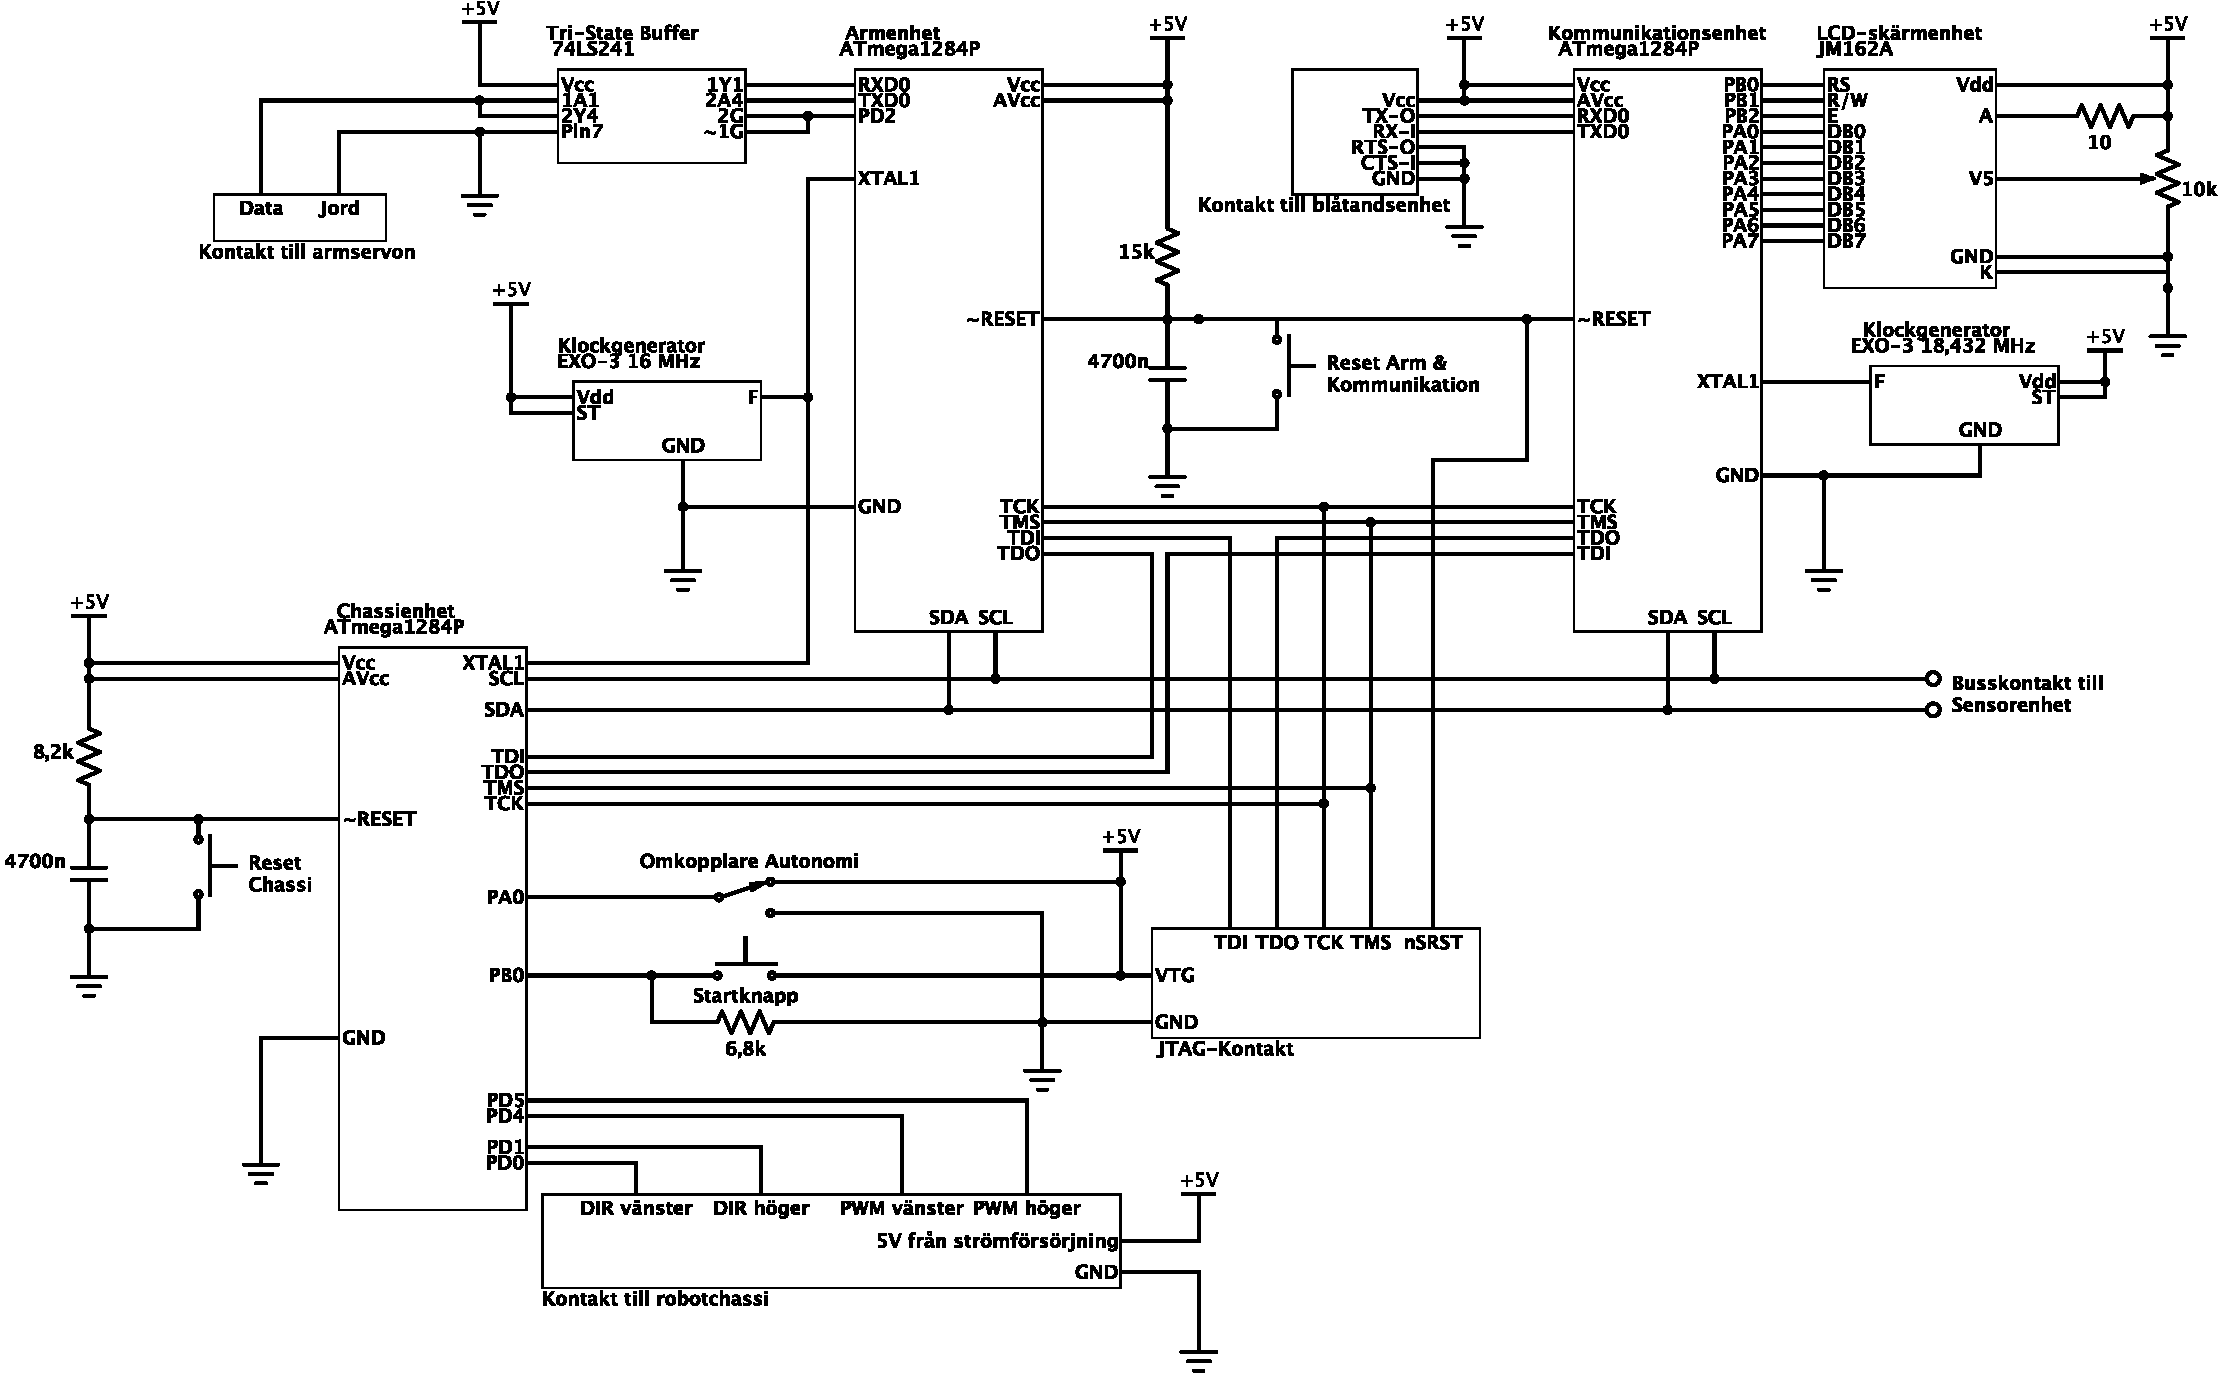
\includegraphics[angle=90,width=0.9\textwidth]{bilder/chassiarmkomm.pdf}
  \emph{\caption{Kopplingsschema över virkortet som innehåller kommunikationsenheten, chassienheten och armenheten.} \label{fig:chassiarmkomm}}
  
\end{figure}


\section{Utdrag från programlistning}
\emph{(ca 5-10 sidor så att vi kan bedöma kodens läsbarhet mm.) och eventuell VHDL-kod}
\section{Övriga bilagor?}


\end{document} 
